\documentclass[10pt, english, xcolor={dvipsnames, table}]{beamer}

% --- 1. Pacchetti Fondamentali (Dallo stile del report) ---
\usepackage[utf8]{inputenc}
\usepackage[T1]{fontenc}
\usepackage[english]{babel}
\usepackage{lmodern} % Font Latin Modern come nel report 
\usepackage{amsmath, amssymb, amsfonts}
\usepackage{graphicx}
\usepackage{tcolorbox}
\usepackage{listings}
\tcbuselibrary{listings}

% --- 2. Definizione Colori (Identici al report)  ---
\definecolor{UniOrange}{rgb}{0.8, 0.4, 0.1}  
\definecolor{UniBlue}{rgb}{0.1, 0.3, 0.7}    
\definecolor{DeepBlue}{rgb}{0, 0.2, 0.4}     
\definecolor{LinkBlue}{rgb}{0.1,0.2,0.9}     

% --- 3. Configurazione Tema Beamer ---
\usetheme{Madrid} % Base solida e pulita
\usecolortheme{whale} % Palette blu di base

% Personalizzazione Colori Beamer
\setbeamercolor{structure}{fg=UniBlue} % Colore titoli e icone 
\setbeamercolor{palette primary}{bg=DeepBlue, fg=white}
\setbeamercolor{palette secondary}{bg=UniBlue, fg=white}
\setbeamercolor{palette tertiary}{bg=UniOrange, fg=white}
\setbeamercolor{titlelike}{parent=palette secondary, fg=white}
\setbeamercolor{block title}{bg=DeepBlue, fg=white} % Blocchi come nel report 
\setbeamercolor{block body}{bg=orange!5} % Sfondo blocchi arancio chiaro 

% --- 4. Stile Listings (Preso dal report) [cite: 10] ---
\lstdefinestyle{mystyle}{
    commentstyle=\color{Green},
    keywordstyle=\color{LinkBlue}\bfseries,
    stringstyle=\color{red!80!black},
    numberstyle=\tiny\color{gray},
    basicstyle=\ttfamily\scriptsize, % Ridotto per le slide
    breaklines=true,
    tabsize=2,
}

\lstdefinestyle{bashstyle}{
    style=mystyle,    
    language=bash,    
    morekeywords={    
        rm, ssh, scp, ls, cd, grep, apt, get, yum, systemctl,
        mv, cp, mkdir, chmod, chown, cat, nano, vim, service, shutdown, ip, netplan, ln, systemctl, restart, VBoxManage, mpirun, touch, docker, hpcc, stress, ng, sysbench, iperf3, iozone
    }
}

% Box per il codice (Stile tcolorbox del report) 
\newtcblisting[auto counter]{codice}[2][]{
    arc=3mm,
    colback=orange!5,
    colframe=orange!80,
    boxrule=0.8pt,
    % ----- Title Options -----
    title={Code \thetcbcounter: #2},
    colbacktitle=DeepBlue,
    coltitle=white,
    fonttitle=\bfseries,
    % ----- LISTINGS Options -----
    listing only,
    listing options={
        style=mystyle, 
        #1
    }
}

% --- 5. Metadati (Presi dal report) [cite: 13, 14] ---
\title[Performance Report]{Performance Report \\ \Large Cloud Computing}
\author[G. Granzotto]{Gabriele Granzotto}
\institute[UniTS]{Università degli studi di Trieste}
\date{\today}
\titlegraphic{
\includegraphics[width=2cm]{settings/units_blue_logo.png}}

\begin{document}

% Slide del Titolo
\begin{frame}
    \titlepage
\end{frame}

% Slide Indice
\begin{frame}{Outline}
    \tableofcontents
\end{frame}

\section{Introduction}
\begin{frame}{Objective}
    \begin{center}
        
\includegraphics[width=2cm]{images/VirtualBox_Logo.png}
        \hspace{0.25cm} {\Huge \textbf{vs}} \hspace{0.25cm}
        
\includegraphics[width=2cm]{images/Docker_Logo.png}
    \end{center}
    \begin{itemize}
        \item \textbf{\color{UniOrange}Goal:} Implementation of parallel clusters: \texttt{VM} vs \texttt{Docker}.
        \item \textbf{\color{UniOrange}Metrics:} Comparative Analysis of CPU, Memory, and Network Usage.
        \item \textbf{\color{UniOrange}Question:} Which technology minimizes virtualization overhead? How much?
    \end{itemize}
\end{frame}

\section{Hardware and Software Setup}
\begin{frame}{Hardware and OS}
    \begin{table}[H]
        \centering
        \begin{tabular}{r|l}
            \color{UniOrange}{CPU}:  & Intel Core i5-8365U 1.60GHz \\
            \color{UniOrange}{RAM}:  & 16GB DDR4                   \\
            \color{UniOrange}{DISK}: & 256GB SSD NVMe
        \end{tabular}
        \caption{Hardware Specification}
        \label{tab:hardware}
    \end{table}
    \begin{itemize}
        \item \textbf{\color{UniOrange}Host OS:} Ubunutu 20.04 LTS (64-bit).
        \item \textbf{\color{UniOrange}Guest OS:} Ubunutu 20.04 LTS (64-bit) for both \texttt{VM} and \texttt{Docker}.
        \item \textbf{\color{UniOrange}Programs:} {\color{UniBlue}Oracle VirtualBox} and {\color{UniBlue}Docker CE}.
        \item \textbf{\color{UniOrange}Equality:} Limited resources to 2 vCPUs and 4GB RAM for both environments to ensure a fair comparison.
    \end{itemize}
\end{frame}

\section{Virtual Machine setup}
\begin{frame}{Virtual Machine Setup: Overview}
    \begin{itemize}
        \item \textbf{\color{UniOrange}Setting OS:} Install the OS, Update, Upgrade and install useful programs and benchmarking tools.
        \item \textbf{\color{UniOrange}Internal Network:} Setting the Internal Network for communication between containers.
        \item \textbf{\color{UniOrange}Shared Filesystem:} Setting a shared folder for data exchange between the host and the VM.
        \item \textbf{\color{UniOrange}Useful Scripts:} Creation of scripts to automate the setup and execution of benchmarks.
    \end{itemize}
\end{frame}

\begin{frame}[fragile]{Virtual Machine Setup: IP Configuration}
    \begin{table}[H]
        \centering
        \begin{tabular}{r|l}
            \color{UniOrange}{Mask}:        & 255.255.255.0  \\
            \color{UniOrange}{Lower Bound}: & 192.168.56.2   \\
            \color{UniOrange}{Upper Bound}: & 192.168.56.199
        \end{tabular}
        \caption{CloudBasicNet}
        \label{tab:ip_settings}
    \end{table}
    \begin{codice}[style=bashstyle]{ssh connection from localhost to master}
        ssh -p 4022 user01@localhost
    \end{codice}
\end{frame}

\begin{frame}[fragile]{Virtual Machine Setup: Network Configuration}
    \begin{codice}[style=bashstyle]{/etc/netplan/50-cloud-init.yaml}
        network:
        version: 2
        ethernets:
        enp0s3:
        dhcp4: true
        enp0s8:
        dhcp4: false
        addresses: [192.168.56.1/24]
    \end{codice}
    \begin{itemize}
        \item \textbf{\color{UniOrange}Netplan:} Configuration of the network interfaces using Netplan.
        \item \textbf{\color{UniOrange}enp0s3:} Interface for NAT connection to the host, configured to obtain an IP address via DHCP.
        \item \textbf{\color{UniOrange}enp0s8:} Interface for the internal network, configured with a static IP address.
    \end{itemize}
\end{frame}

\begin{frame}[fragile]{Virtual Machine Setup: Hosts File}
    \begin{codice}[style=bashstyle]{hosts name change}
        127.0.0.1 localhost
        127.0.1.1 master
        192.168.56.1 master

        192.168.56.2 node02
        192.168.56.3 node03
        192.168.56.4 node04
        192.168.56.5 node05
        192.168.56.6 node06
        192.168.56.7 node07
        192.168.56.8 node08
        192.168.56.9 node09

        # The following lines are desirable for IPv6 capable hosts
        ::1     ip6-localhost ip6-loopback
        fe00::0 ip6-localnet
        ff00::0 ip6-mcastprefix
        ff02::1 ip6-allnodes
        ff02::2 ip6-allrouters
    \end{codice}
\end{frame}

\begin{frame}[fragile]{Virtual Machine Setup: DNS Configuration}
    \begin{codice}[]{/etc/dnsmasq.conf}
        interface=enp0s8
        bogus-priv
        bind-interfaces
        cache-size=1000
        resolv-file=/etc/resolv.dnsmasq
        listen-address=127.0.0.1,192.168.56.1
        log-queries
        dhcp-range=192.168.56.2,192.168.56.10,12h
    \end{codice}

    \begin{codice}[]{/etc/resolv.conf}
        nameserver 192.168.56.1
        search .
    \end{codice}
\end{frame}

\begin{frame}[fragile]{Virtual Machine Setup: SSH Configuration}
    \begin{codice}[style=bashstyle]{ssh public key}
        ssh-keygen
        mkdir ~/.ssh
        chmod 700 ~/.ssh
        cat ~/id_rsa.pub >> ~/.ssh/authorized_keys
        chmod 644 ~/.ssh/authorized_keys
    \end{codice}
    \begin{codice}[style=bashstyle]{scp command}
        scp -P 4022 /[path]/[to]/[my]/[file] \
        user01@localhost:/[path]/[to]/[send]/
    \end{codice}
\end{frame}

\begin{frame}[fragile]{Virtual Machine Setup: NFS Configuration}
    \begin{codice}[style=bashstyle]{/etc/exports}
        ...
        /shared/  192.168.56.0/255.255.255.0(rw,sync,no_root_squash,no_subtree_check)
        ...
    \end{codice}
    \begin{codice}[style=bashstyle]{/etc/exports}
        sudo systemctl enable nfs-kernel-server
        sudo systemctl restart nfs-kernel-server
        sudo mkdir /shared/data /shared/home
        sudo chmod 777  /shared/data /shared/home
    \end{codice}
\end{frame}

\begin{frame}[fragile]{Virtual Machine Setup: Useful Scripts}
    \begin{codice}[style=bashstyle]{upVM.sh}
        #!/bin/bash
        echo "Power On of the VM cluster..."
        VBoxManage startvm "Ubuntu_VM_Master" --type headless
        VBoxManage startvm "Ubuntu_VM1" --type headless
        VBoxManage startvm "Ubuntu_VM2" --type headless
        echo "Power On command send successfully to all VMs."
    \end{codice}
    \begin{codice}[style=bashstyle]{downVM.sh}
        #!/bin/bash
        echo "Shut down of the VM cluster..."
        VBoxManage controlvm "Ubuntu_VM_Master" acpipowerbutton
        VBoxManage controlvm "Ubuntu_VM1" acpipowerbutton
        VBoxManage controlvm "Ubuntu_VM2" acpipowerbutton
        echo "Shutdown command send successfully to all VMs."
    \end{codice}
\end{frame}

\section{Container setup}
\begin{frame}{Container Setup: Overview}
    \begin{itemize}
        \item \textbf{\color{UniOrange}Container Structure:} Design a multi-container architecture with a master and multiple worker containers.
        \item \textbf{\color{UniOrange}Docker Compose:} Use Docker Compose to orchestrate the multi-container application.
        \item \textbf{\color{UniOrange}Master Node:} Create a Dockerfile for the master node, including necessary software and configurations.
        \item \textbf{\color{UniOrange}Client Node:} Same for the client node, ensuring it can communicate with the master and run benchmarks.
        \item \textbf{\color{UniOrange}SSH problems \& Strategy:} Security considerations for SSH key passing between containers and from host to master.
    \end{itemize}
\end{frame}

\begin{frame}[fragile]{Container Setup: Container Structure}
    \begin{codice}[]{Docker project structure}
        Docker-Configuration/
        |
        +--docker-compose.yml
        |
        +--master/
        |  |
        |  +-- Dockerfile
        +--nodes/
        |  |
        |  +-- Dockerfile
        +--shared_data/
    \end{codice}
    \begin{codice}[style=bashstyle]{docker compose commands}
        docker compose build --no-cache
        docker compose up -d
        docker compose down
        docker exec - it node bash
    \end{codice}
\end{frame}

\begin{frame}[fragile]{Container Setup: Docker Compose}
    \begin{center}
        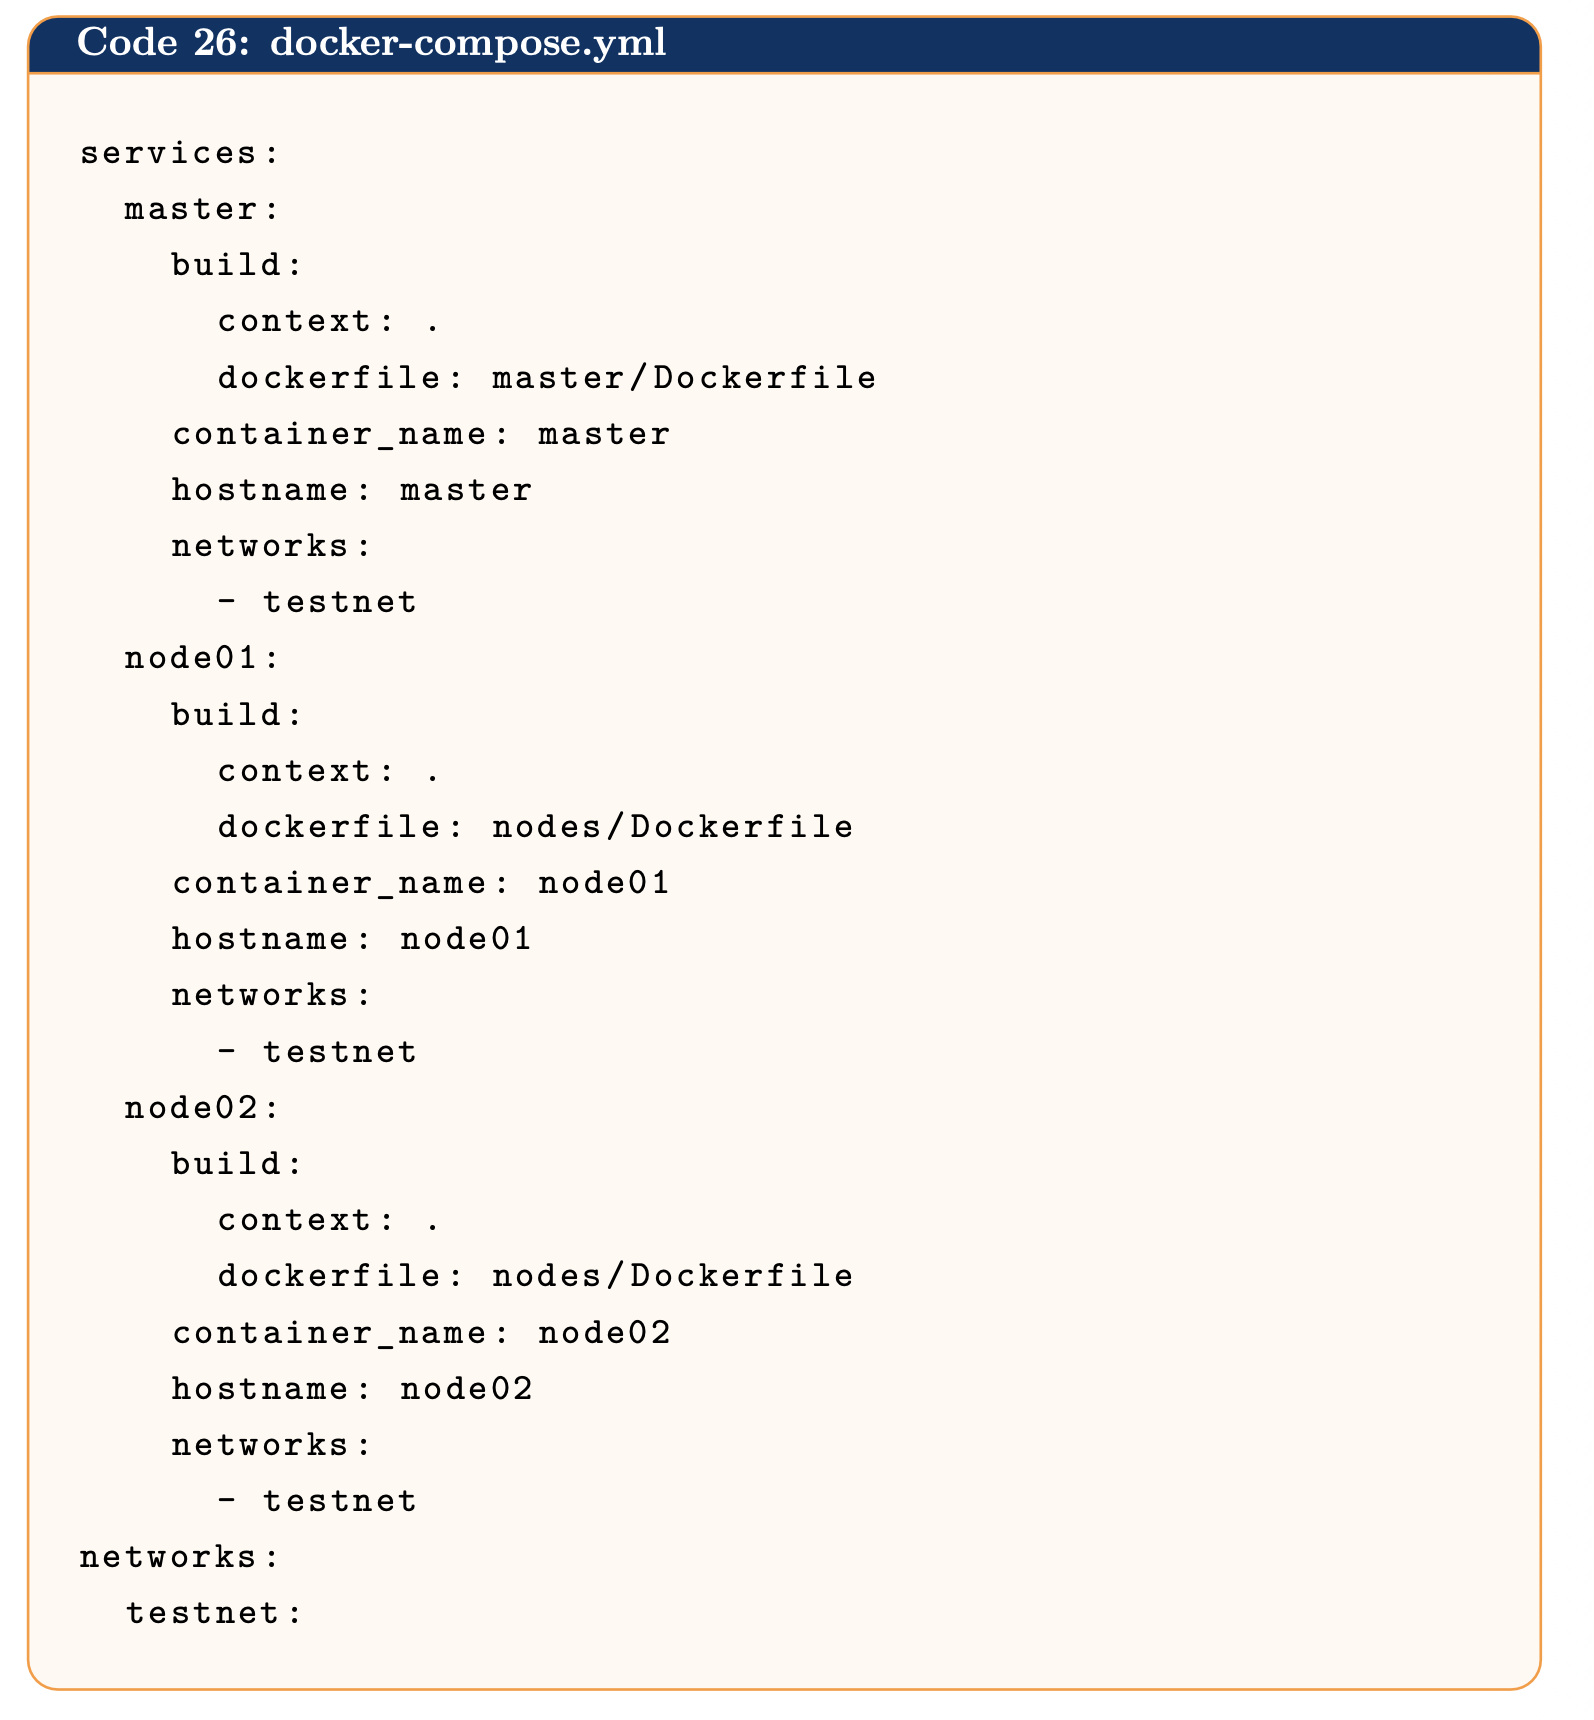
\includegraphics[width=0.6\textwidth]{images/docker_compose.png}
    \end{center}
\end{frame}

\begin{frame}[fragile]{Container Setup: Docker Compose - Shared File System}
    \begin{codice}[style=bashstyle]{docker-compose.yml}
        services:
        master:
        ...
        volumes:
        - ./shared_data:/data

        node01:
        ...
        volumes:
        - ./shared_data:/data

        node02:
        ...
        volumes:
        - ./shared_data:/data
        ...
        volumes:
        ./shared_data:
    \end{codice}
\end{frame}

\begin{frame}[fragile]{Container Setup: Docker Compose - Network Config}
    \begin{codice}[style=bashstyle]{docker-compose.yml}
        services:
        master:
        ...
        cpus: '2.0'
        mem_limit:2G

        node01:
        ...
        cpus: '2.0'
        mem_limit:2G

        node02:
        ...
        cpus: '2.0'
        mem_limit:2G
        ...
        volumes:
        ./shared_data:
    \end{codice}
\end{frame}

\begin{frame}[fragile]{Container Setup: Master Node}
    \begin{codice}[style = bashstyle]{master/Dockerfile}
        FROM ubuntu:24.04
        ENV DEBIAN_FRONTEND=noninteractive \
        TZ=Europe/Rome

        RUN apt-get update && \
        apt-get install -y --no-install-recommends \
        nano vim curl wget build-essential \
        software-properties-common \
        hpcc mpich stress-ng sysbench iozone3 iperf3 netcat-openbsd \
        openssh-client \
        && apt-get clean && rm -rf /var/lib/apt/lists/*

        RUN ssh-keygen -f /root/.ssh/id_rsa -N "" \
        && echo "Host *" > /root/.ssh/config \
        && echo "    StrictHostKeyChecking no" >> /root/.ssh/config \
        && echo "    UserKnownHostsFile /dev/null" >> /root/.ssh/config \
        && chmod 600 /root/.ssh/config

        WORKDIR /root/
        CMD ["/bin/bash"]
    \end{codice}
\end{frame}

\begin{frame}[fragile]{Container Setup: Client Node}
    \begin{codice}[style=bashstyle]{some ssh command}
        RUN mkdir /var/run/sshd \
        && echo 'root:root' | chpasswd \
        && sed -i 's/#PermitRootLogin prohibit-password/PermitRootLogin yes/' /etc/ssh/sshd_config \
        && sed -i 's/#PasswordAuthentication yes/PasswordAuthentication yes/' /etc/ssh/sshd_config \
    \end{codice}
    \begin{codice}[style=bashstyle]{node CMD}
        CMD ["/usr/sbin/sshd -D"]
    \end{codice}
\end{frame}

\begin{frame}{Container Setup: SSH Key Passing Strategy - Problem}
    \begin{center}
        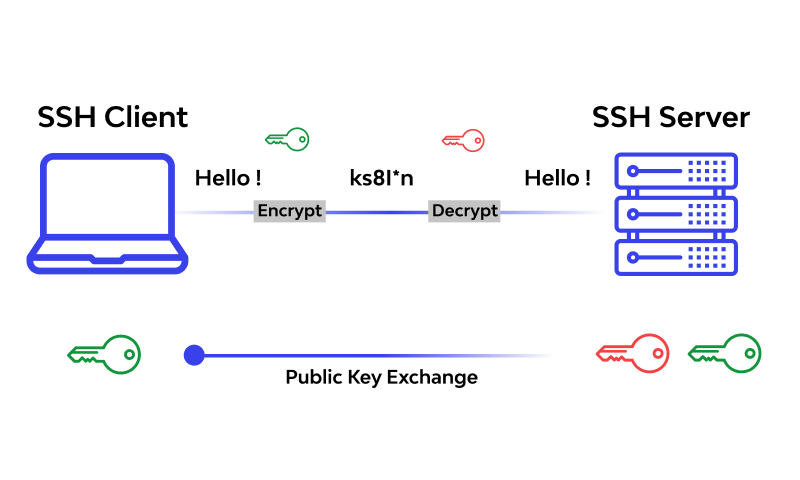
\includegraphics[width=0.7\textwidth]{images/ssh_image.png}
    \end{center}
    The standard generation of SSH keys works but:
    \begin{itemize}
        \item process cannot be automated during the image build.
        \item security problems sharing private keys.
    \end{itemize}
\end{frame}

\begin{frame}[fragile]{Container Setup: SSH Key Passing Strategy - Healthcheck}
    \begin{codice}[style=bashstyle]{healthcheck}
        services:
        master:
        ...
        healthcheck:
        test: ["CMD", "test", "-f", "/data/id_rsa.pub"]
        interval: 1s
        timeout: 60s
        start_period: 3s
        ...
        node01:
        ...
        depends_on:
        master:
        condition: service_healthy
        ...
        node01:
        ...
        depends_on:
        master:
        condition: service_healthy
        ...
    \end{codice}
\end{frame}

\begin{frame}[fragile]{Container Setup: SSH Key Passing Strategy - Script}
    \begin{codice}[style=bashstyle]{node CMD (snippet)}
        CMD ["/bin/bash", "-c", "/root/setup.sh && /usr/sbin/sshd -D"]
    \end{codice}
    \begin{codice}[style=bashstyle]{script.sh}
        #!/bin/bash
        mkdir -p /root/.ssh
        chmod 700 /root/.ssh
        touch /root/.ssh/authorized_keys
        chmod 600 /root/.ssh/authorized_keys
        cat /data/id_rsa.pub >> /root/.ssh/authorized_keys
    \end{codice}
    \begin{codice}[style=bashstyle]{password client (snippet)}
        RUN mkdir /var/run/sshd \
        && echo 'root:\$(openssl rand -base64 12)' | chpasswd \
    \end{codice}
\end{frame}

\section{Performance Test}
\begin{frame}{Performance Test: Overview}
    \begin{center}
        \begin{figure}
            
\includegraphics[width=0.25\textwidth]{images/benchmark.png}
            \caption{free-to-use image credit to Eucalyp}
            \label{fig:benchmark}
        \end{figure}
    \end{center}
    \begin{itemize}
        \item \textbf{\color{UniOrange}CPU:} HPL, FFT, starDGEMM, stress-ng, sysbench.
        \item \textbf{\color{UniOrange}Memory:} MPI random access, starSTREAM triad, stress-ng, sysbench.
        \item \textbf{\color{UniOrange}Disk:} iozone.
        \item \textbf{\color{UniOrange}Network:} iperf3.
    \end{itemize}
\end{frame}


\begin{frame}{Key Takeaways}
    \vspace{0.3cm}
    \begin{alertblock}{Important}
        L'ambiente \texttt{fragile} è necessario quando si usa il codice nelle slide.
    \end{alertblock}
    \begin{block}{Key Objective}
        Mantenere la coerenza visiva tra il documento scritto e la presentazione orale.
    \end{block}
\end{frame}

\end{document}